\documentclass[]{report}
\usepackage{tikz}
\newcommand{\inputtikz}[2]{%  
	\scalebox{#1}{\input{#2}}  
}
\usepackage[english]{babel}
\usepackage[utf8x]{inputenc}
\usepackage{amsmath}
\usepackage{graphicx}
\usepackage{hyperref}
\usepackage[colorinlistoftodos]{todonotes}
\usepackage{listings}
\usepackage{color}
\usepackage{amsmath}
\usepackage{amsfonts}
\usepackage{mathtools}
\usepackage{graphicx}
\usepackage{caption}
\definecolor{dkgreen}{rgb}{0,0.6,0}
\definecolor{gray}{rgb}{0.5,0.5,0.5}
\definecolor{mauve}{rgb}{0.58,0,0.82}
\renewcommand{\thesection}{\arabic{section}}
%opening

\begin{document}
	
	\begin{titlepage}
		
		\newcommand{\HRule}{\rule{\linewidth}{0.5mm}} 
		
		\center 
		
		\textsc{\LARGE Université de Technologie de Compiègne}\\[1.5cm]
		\textsc{\Large NF26}\\[0.5cm] 
		\textsc{\large Data Warehouse}\\[0.5cm]
		
		\HRule \\[0.4cm]
		{ \huge \bfseries Rendu TP Cassandra}\\[0.4cm] 
		\HRule \\[1.5cm]
		
		
		\begin{center}
			Zineb \textsc{SLAM} 
		\end{center}
		
		{\large \today}\\[2cm] 
		
		
\includegraphics[width=40mm]{Figures/utc.jpg}\\ % 
		
		\vfill
		
	\end{titlepage}
	\lstset{frame=tb,
		language=SQL,
		aboveskip=3mm,
		belowskip=3mm,
		showstringspaces=false,
		framexleftmargin=5mm,
		columns= fixed,
		numbers = left,
		basicstyle={\small\ttfamily},	
		numberstyle=\tiny\color{gray},
		keywordstyle=\color{blue},
		commentstyle=\color{dkgreen},
		stringstyle=\color{mauve},
		breaklines=true,
		breakatwhitespace=true,
		tabsize=3
	}
	
	
	\begin{abstract}
		Dans cette deuxième partie du TP de NF26 nous allons traiter de gros volumes de données avec Cassandra. Nous allons d'abord commencer par décrire nos données, puis présenter une modélisation des Datamarts et pour finir nous allons expliquer comment nous avons exploités ces données. Vu le cours temps dont nous avons disposé et la nouveauté de cette méthode de stockage ainsi que les langages CQL et Python, nous  n'avons ne sommes restreint à une seule méthode d'analyse statistique. Néanmoins nous avons essayé de détailler au maximum les méthodes appliquées en soulignant les prochaines démarches  à prendre pour la continuité du projet. Comme le contexte du projet ne nous pas été définie, il a fallu émettre des hypothèses au cours de notre étude pour argumenter notre modélisation.
	\end{abstract}
	
	\tableofcontents
	
	
	\pagebreak
	
	
	\section{Description des Données}
	Nous disposons d'un ensemble de données précis décrivant l'année complète (du 01/07/2013 au 30/06/2014) des trajectoires effectuées par 442 taxis dans la ville de Porto au Portugal (c'est-à-dire 3Gb de données Stocké dans un seul fichier CSV). Ces taxis fonctionnent à travers un centre d'expédition de taxi, en utilisant des terminaux de données mobiles installés dans les véhicules (GPS et autres). Chaque trajet est caractérisé en trois catégories: A) basé sur le taxi centralisé, B) à base de stand ou C) sur n'importe quelle rue. Chaque entrée de données correspond à un un trajet complété. Il contient au total 9 attributs, décrits comme suit:
	
	\begin{itemize}
		\item \textbf{TRIP\_ID}: est un String qui identifie chaque trajet du taxi
		\item \textbf{CALL\_TYP}E est un caractère désignant comment la demande de service a été faite
		\begin{itemize}
			\item A appel du centre/station
			\item B une demande directe au taxi dans un point d'arrêt
			\item C une demande faite dans n'importe quel point de la rue
		\end{itemize}
		\item \textbf{ORIGIN\_CALL} est un entier contenant le numéro de téléphone que le client a utilisé pour demander un service. Cet attribut est défini que si CALL\_TYPE=A si non la valeur est nulle
		\item \textbf{ORIGIN\_STAND}: est une identifiant du point d'arrêt/station du départ de du taxi, si CALL\_TYPE=B si non la valeur est nulle
		\item \textbf{TAXI\_ID}: est entier contenant  l'identifiant du taxi effectuant le trajet
		\item \textbf{TIMESTAMP}: est un entier désignant la date et heure du début du trajet en UNIX TimeStamp.
		\item \textbf{DAYTYPE}: est un caractère identifiant le type de jour du début du trajet. Il prend une de ces valeur:
		\begin{itemize}
			\item 'A' pour un jour normal (jour de semaine ou week-end)
			\item 'B' si le voyage a commencé en un jour de  vacances ou un jour de fête.
			\item 'C' si le voyage a commencé la veille d'un jour de type B
		\end{itemize}
		\item \textbf{MISSING\_DATA} est un booléen qui est \textit{TRUE} si la suite de localisations du taxi par  GPS est complète, \textit{FALSE} si des coordonnées sont manquantes.
		\item \textbf{POLYLINE} est une suite de coordonnées enregistrés par le GPS du taxi  toutes les 15 secondes; sous la forme [longitude, latitude]. La première entrée est le point de départ tandis que la dernière est la destination du voyage.
	\end{itemize}
	
	
	\section{Modélisation}
	Nous avons identifié 5 dimensions pour notre base de données:
	\subsection{Dimensions}
	Notre modélisation est représentée par le diagramme ci-dessous:
	\begin{center}
		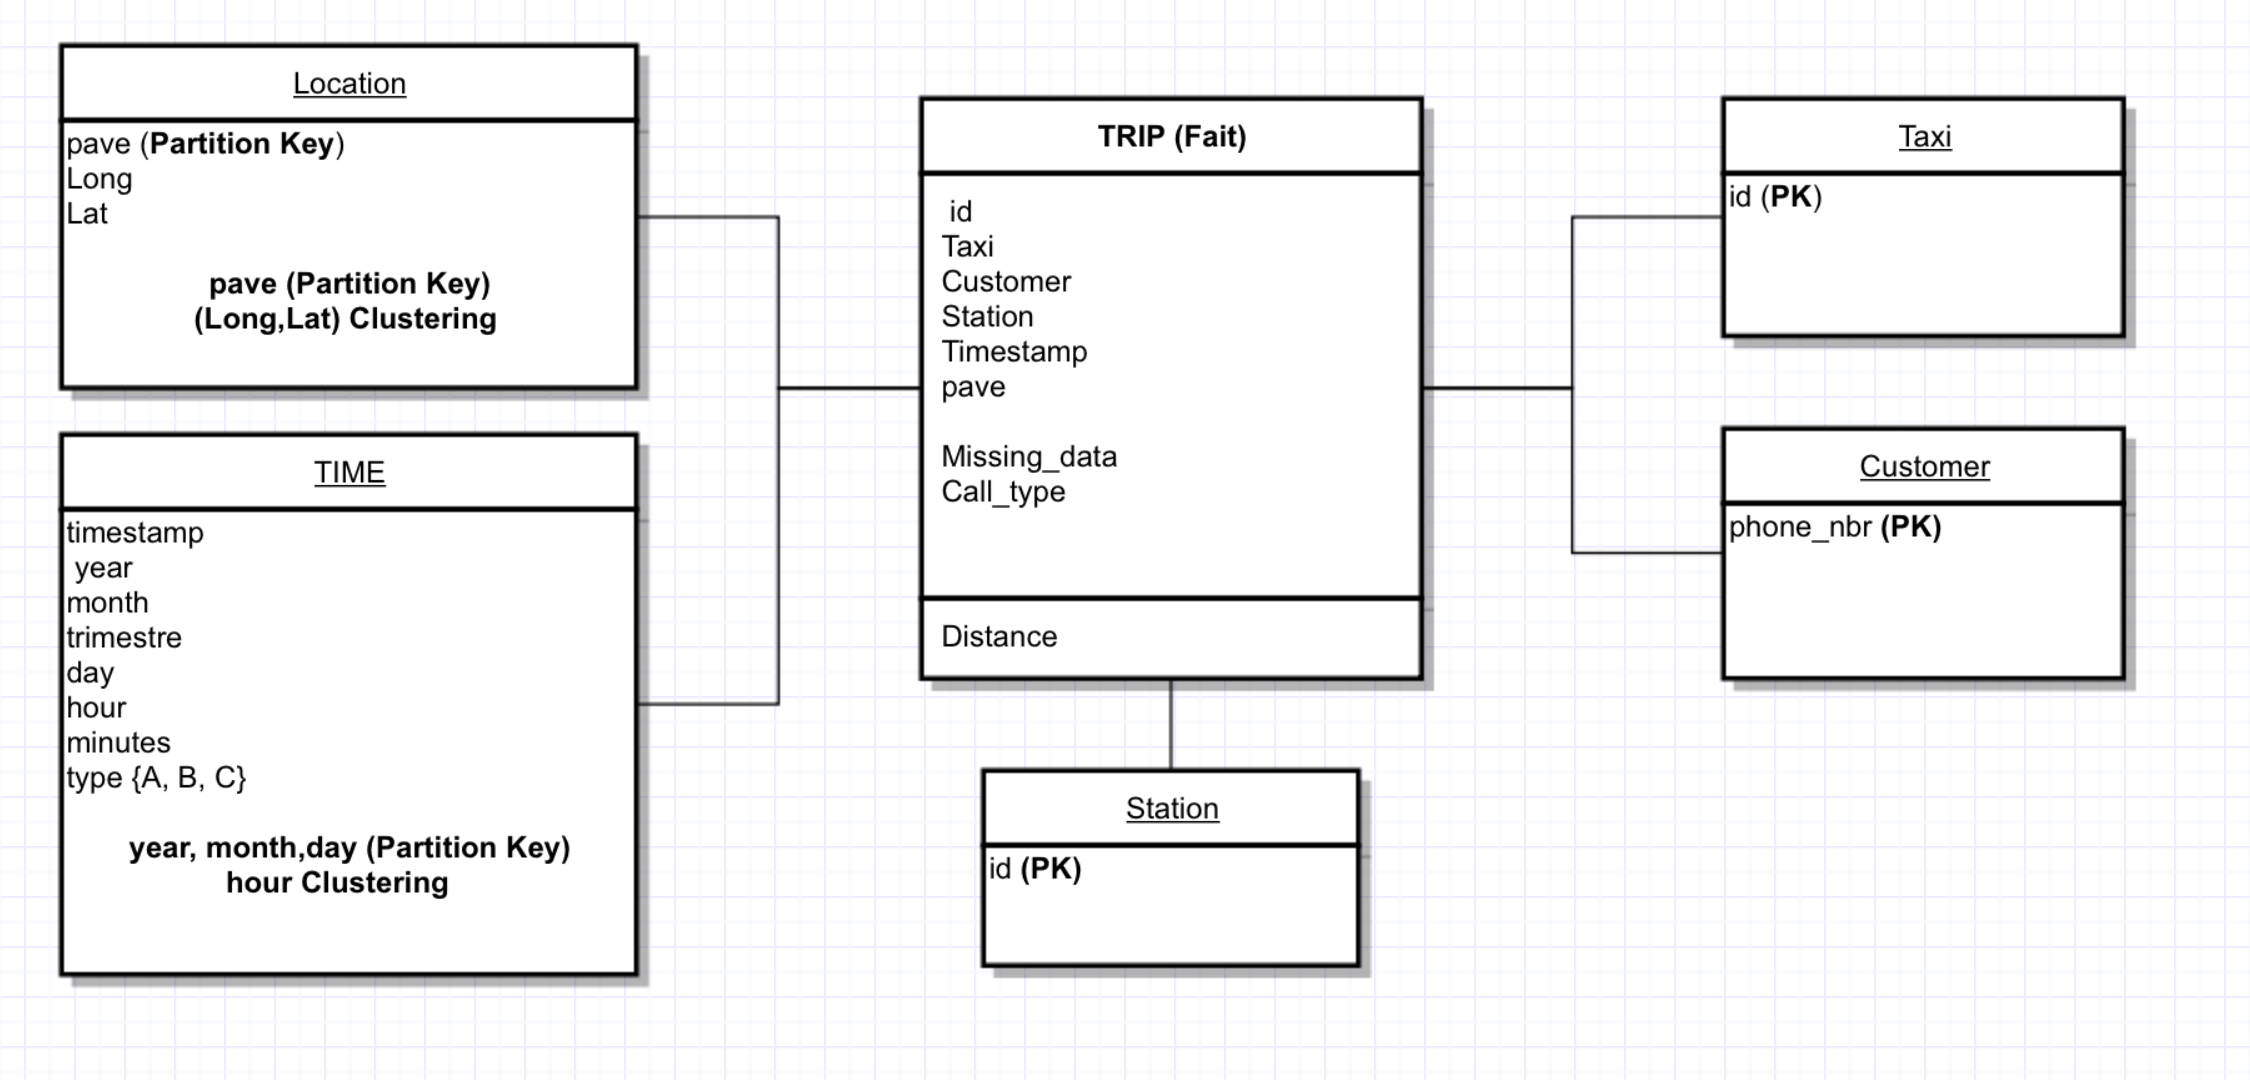
\includegraphics[width=120mm]{Figures/modele.png}
		\captionof{figure}{Modelisation de la Base de Données}
		\label{fig:y=6}
	\end{center}
	Les dimensions sont:
	\begin{itemize}
		\item \textbf{Géographique}: notre dimension géographique est formée d'une table de localisation. Dans cette table nous avons implémenté un pavé comme partition key ensuite nous avons ordonné chaque partition par longitude et latitude. Nous allons détailler le calcul de ce pavé dans les sections suivantes.
		\item \textbf{Temporelle}: notre dimension Temporelle est composée d'une seule table Date. Dans nos données nous avons uniquement le TimeStamp et type de jour. Mais il sera pertinent d'avoir les attributs années, mois, jour et heure. Pour avoir une partition suffisamment grande mais qui ne croît pas indéfiniment on a choisit de partitionner par année, par mois et par jour. Nous justifierons davantage ce choix dans la section suivante.
		\item \textbf{Taxi}: elle est composée d'une table Taxi avec tous les id des Taxi
		\item \textbf{Station} est composée d'une table Station avec les id de chaque station (ce qui correspond à origin\_stand)
		\item \textbf{Client}  est composée d'une table avec comme attribut un id qui correspond au numéro de téléphone du client (origin\_call)
		
	\end{itemize}
	\subsection{Faits}
	Nous avons modélisé nos table de faits en répondant à la question: "Que voudrai je afficher ou représenter?". Ainsi dans chacune des sous-parties qui suit nous allons commencer par énoncer la ou les  questions ensuite de trouver la modélisation de la table de fait pour y répondre. \\
	\subsubsection{Attributs}
	Notons que toutes nos tables de faits ont les mêmes attributs qui correspondent en majorité à ceux du fichier csv. Nous avons décidé de garder le maximum d'information pour que notre modèle soit extensible dans le temps. C'est a dire si on voudrait répondre à d'autres sous-question ou obtenir plus d'informations on ne sera pas amené à re-modéliser notre table de fait. Nous avons décidé dans le cadre de ce TP de ne pas insérer la liste Polyline dans notre table de fait et ce pour 2 raisons; la première est que cette liste va considérablement augmenter la taille de notre base de données alors que nous ne l'exploiterons pas dans nos questions. La seconde est que  le matériel dont nous disposons à l'UTC pourrait ne pas supporter une aussi grande taille de partition. Il faudra quand même  garder en tête que ceci n'est qu'une première modélisation et que plus tard si ce modèle sera ré-utilisé il faudra penser à rajouter cette information de trajet dans au moins une des tables pour des raisons d'évolutivité.
	\subsubsection{Question 1}
	\begin{itemize}
		\item Quel est le nombre de trajets par mois et par jour?
		\item Comment le nombre de trajets évolue au cours de la journée?
		\item Quelle est la distance totale parcourue par période?
	\end{itemize}
	
	Il est bien claire d'après ces questions qu'on voudrait obtenir des informations par rapport à une date et donc on devrait avoir une partition par date. La question qui se pose ici est quels sont les attributs à regrouper dans la clés de partitionnement. Comme il a déjà été cité dans la modélisation de la dimension date. Il faut que notre partition n'augmente pas indéfiniment au cours du temps et qu'elle ne soit pas trop fine non plus. On a alors hésité entre (year,month) et (year, month, day).  En choisissant (year,month) nous avons 12 partitions par an avec environ 400,000 entrées par partition. Tandis qu'avec (year,month,day) nous avons 365 partitions par an et environ 6000 entrée par partition. Comme on ne connaît pas a priori la taille des nœuds dans le serveur on ne peut pas trancher entre les 2 propositions. Mais si on  suppose que nos données vont augmenter et qu'on aura une croissance de trajets au cours des années on choisira plutôt la clés de partitionnement (year, month,day).  De plus le fait de l'utilisation de 3 colonnes au lieu de 2 pour acheminer vers une partition peut diminuer les \textit{hotspots}. Ainsi on aura une partition pour chaque jour de l'année. Cette partition sera ordonnée par heure puis par trip\_id pour différencier entre 2 trajets qui ont commencé à la même date et heure. Autre remarque, on ne connaît pas le nombre de serveurs dont on dispose mais avec 365 partitions par an il nous faut au moins 10 serveur pour avoir 36 partitions par serveur . Ci-dessous la modélisation de notre table de fait. 
	\begin{center}
		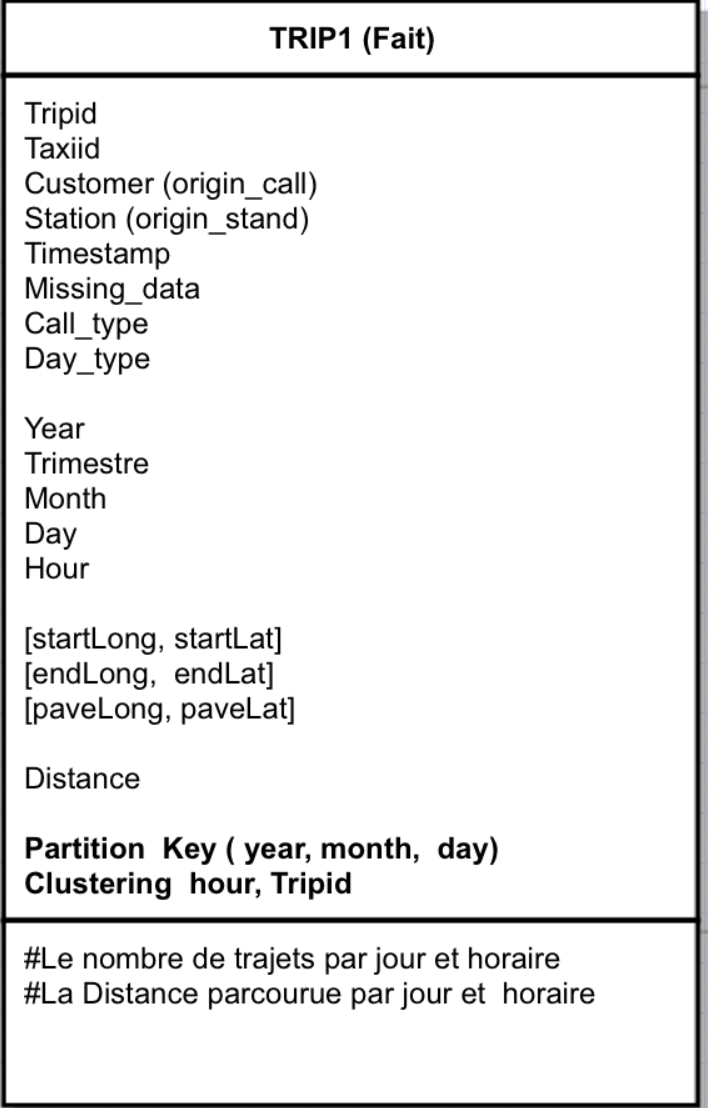
\includegraphics[width=65mm]{Figures/Trip1.png}
		\captionof{figure}{Modélisation de la table de fait Trip1}
		\label{fig:y=6}
	\end{center}
	
	
	\subsubsection{Question 2}
	\begin{itemize}
		\item Quels sont les trajets/ ou le nombre de trajets qui partent d'un pavé entre 2 intervalles de temps( par exemple entre le 10 Juillet 2013 et le 10 Septembre 2013)?
	\end{itemize}
	Dans cette modélisation nous utilisons le pavé pour regrouper les coordonnées de départ des trajets. Nous arrondissons le pavé au dixième près, c'est a dire $pave_{longitude} = (longitude*10)/10, pave_{latitude} = (latitude*10)/10$. Nous avons trouvé plus judicieux d'utiliser comme clés partitionnement (pavé, year) plutôt que (pave, year, month) car avec la deuxième nous aurons 12 fois plus de partitions par année ce qui peut être considérablement lourd comme on a un grand nombre de pavé. Ensuite nous ordonnons les données par month, day, hour et enfin Tripid pour différencier les trajets. 
	
	
	\begin{center}
		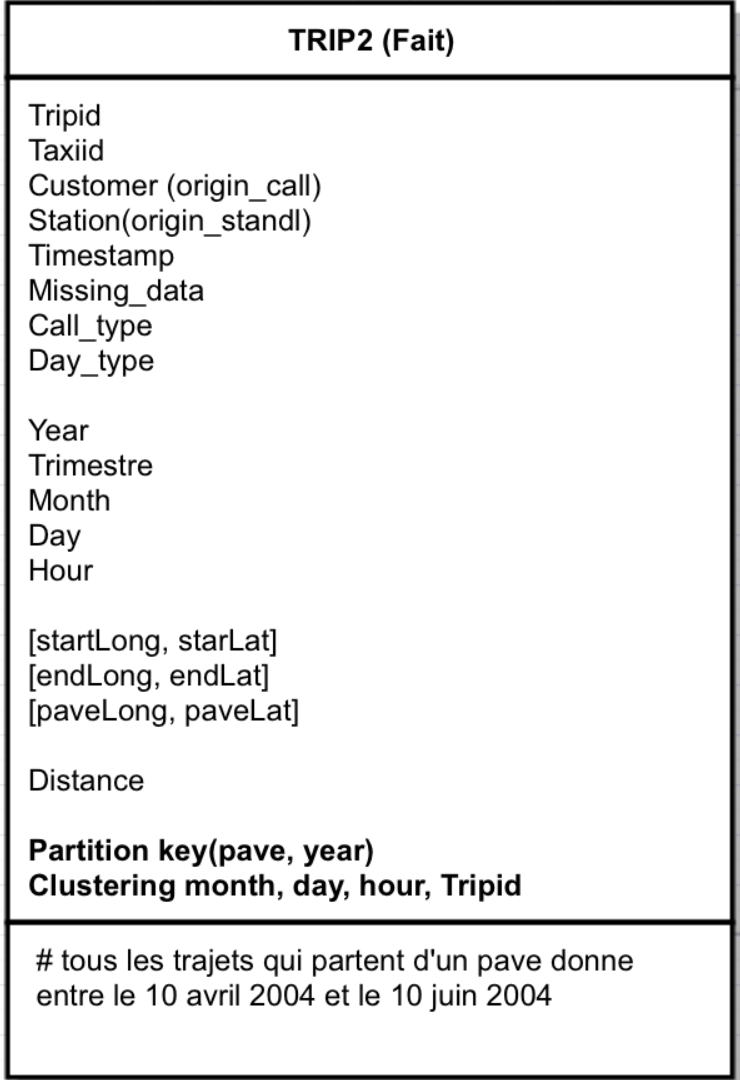
\includegraphics[width=65mm]{Figures/Trip2.png}
		\captionof{figure}{Modélisation de la table de fait Trip2}
		\label{fig:y=6}
	\end{center}
	\subsubsection{Question 3}
	\begin{itemize}
		\item Le meilleure Taxi du mois 
		\item  Nombre moyen de trajet par Taxi
	\end{itemize}
	
	Pour répondre à des question spécifiques a chaque Taxi, il est évident qu’il faut partitionner par l'id du Taxi. Nous avons ensuite considéré le partitionnement par année et par mois. Ainsi si un Taxi fait en moyenne 10 trajets par jour notre partition aura une taille de 3650 ce qui est raisonnable. Le seule inconvénient ici est qu'on aura une partition pour chaque taxi et donc un 442 partitions; il serait donc mieux d'avoir plusieurs serveur pour pouvoir les partager.
	
	\begin{center}
		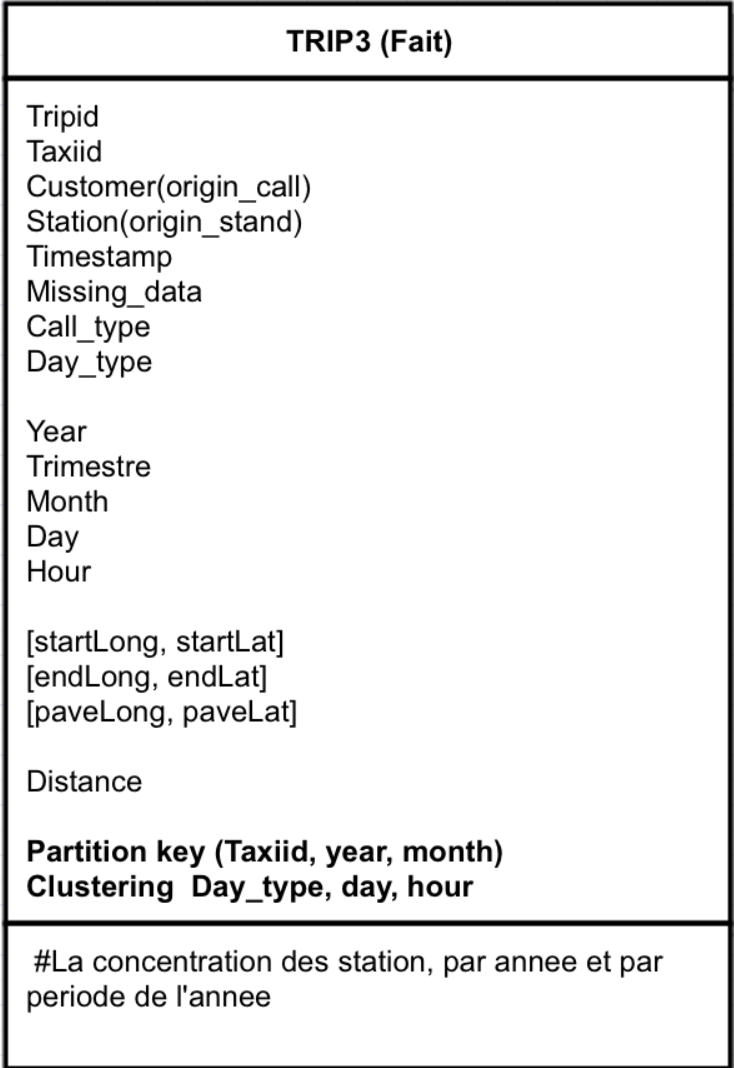
\includegraphics[width=65mm]{Figures/Trip3.png}
		\captionof{figure}{Modélisation de la table de fait Trip3}
	\end{center}
	\subsubsection{Question 4}
	\begin{itemize}
		\item La concentration des stations par année, mois , type de jour
		\item  les stations les plus fréquentées
	\end{itemize}
	On suit ici le même principe que pour les Taxi. Nous partitionnons par l'id de la station, l'année et le mois. Nous ne sommes pas allés jusqu'à partitionner par  jour parce qu'en exploitant les données mises à disposition nous remarquons qu'il n'y' a pas vraiment énormément de trajets de type B.
	
	\begin{center}
		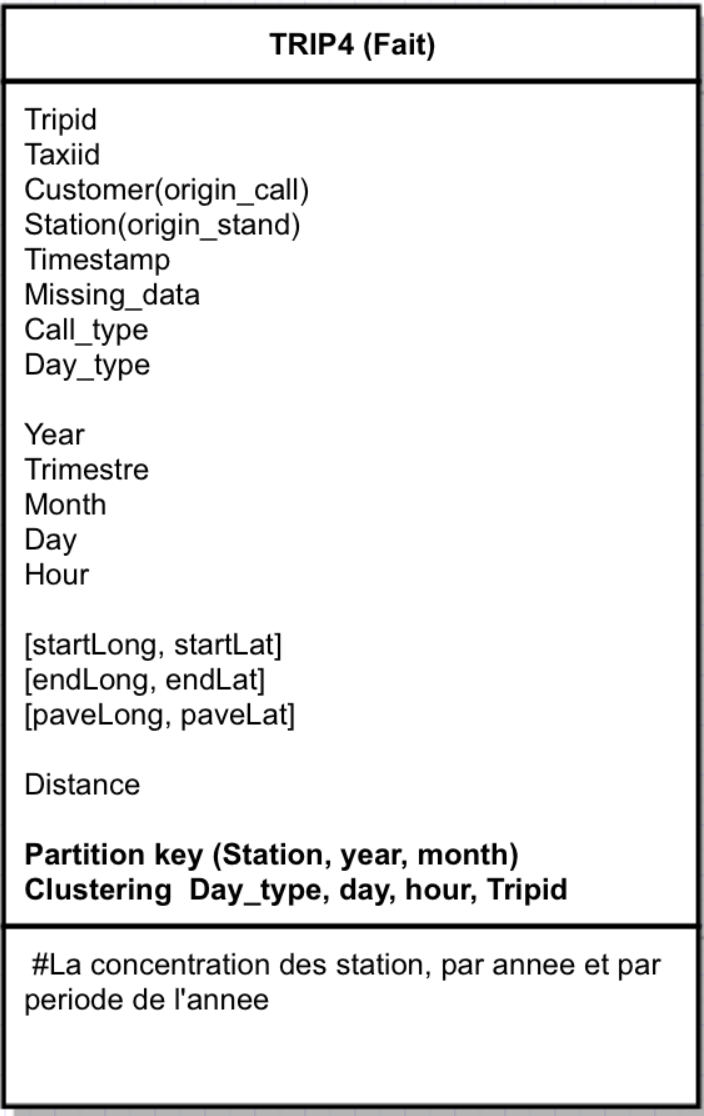
\includegraphics[width=65mm]{Figures/Trip4.png}
		\captionof{figure}{Modélisation de la table de fait Trip4}
	\end{center}
	
	\subsubsection{Question 4}
	\begin{itemize}
		\item Le meilleur client
		\item Les destinations favorites d'un client
		\item Les jours ou types de jours ou un client utilise le plus les taxi
	\end{itemize}
	Ce modèle a été proposé pour exploiter les données pour des fins commerciales. En effet on pourrait se demander quels sont les trajets préférés d'un client pour qu'on puisse envoyer a ces derniers des messages de promotions ou de réductions. Ceci est utilise par exemple par Uber ou Lyft.  Nous pourrons aussi étudier les trajets d'un client afin de prédire ses prochains déplacements et lui proposer de bons plans. Nous allons donc partitionner dans ce cas par idClient (le numéro de téléphone) et l'année. Cette solution n'a pas été mise en place dans la suite par faute de temps et aussi parce que nous n'avons pas autant d'informations sur les clients (c'est à dire un client peut prendre un taxi sans appeler et donc on ne saura pas que c'est lui), mais on a trouvé judicieux de la mentionner pour la suite du projet.
	
	
	\section{Nettoyage et Insertion des données en Python}
	\subsection{Nettoyage}
	Nous avons commencé par parsser le fichier csv en gardant les même types que ceux dans la description des données.  Nous avons parssé la liste de GPS polyline pour n'en garder que les coordonnées de départs et d'arrivée. Nous avons aussi remplacé tous les attributs nuls de origin\_call et origin\_stand par 0 lorsqu'ils sont vides.
	\subsection{Insertion}
	Une fois que nos données sont nettoyées l'insertion n'est pas difficile du moment qu'on fait attention à bien faire les conversions des types. Pour éviter de faire la requête d'insertion ligne par ligne on pourrait utiliser les \textit{BATCH STATEMENT} ou on pourrait insérer chaque 500 lignes par exemple. Le code avec le \textit{BATCH} est mis en commentaire à la fin du fichier d'insertion \textit{taxi.py} en annexe. \\
	Dans notre code on inséré dans les tables stations et Taxi au même temps qu'on insère dans les tables de faits; mais l'idéal était de faire cette insertion après avoir récupéré les id dans un set. En effet le set en Python n'autorise pas de doublons. On fera donc moins de requêtes d'insertion.
	
	
	\section{Exploitation et Visualisation des données}
	\subsection{Trip1}
	Nous interrogeons ici notre table de fait Trip1 pour répondre aux questions posées dans la section précédente. Comme notre clés de partitionnement est (year,month,day) il faut que notre requête \textit{SELECT} contienne des conditions sur ces 3 attributs avec le \textit{WHERE}. Dans un premier temps pour obtenir l'évolution du nombre de trajet par heure nous avons utilisé la requête suivante:
	\begin{lstlisting}
	SELECT hour, COUNT(tripid) as nb FROM TRIP1 WHERE year=2013 AND month=9 AND day=9 GROUP by hour
	\end{lstlisting}
	Ensuite nous avons décidé d'opter le \textit{GROUP BY} car celui alourdit la requête en filtrant la partition. Nous récupérons donc une requête avec tous les trajets pour toutes les heures, et comme nous avons définit les heures comme clés de clustering le résultat sera trié par ordre croissant des heures, il suffira donc juste de compter le nombre de trajets. Notre nouvelle requête devient alors:
	\begin{lstlisting}
	SELECT day, hour, tripid FROM TRIP1 WHERE year=2013 AND month=9 AND day=9
	\end{lstlisting}
	Les résultats pour le nombre de trajets par heure et la distance parcourue par heure pour le 09/09/2013 sont représentés graphiquement ci-dessous:\\
	\begin{minipage}{.5\textwidth}
		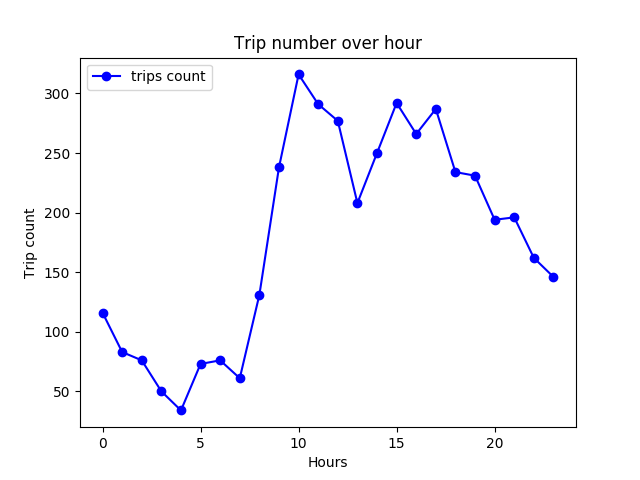
\includegraphics[width=75mm]{Figures/trips_by_day.png}
		\captionof{figure}{Evolution du nombre de trajets par heure}
	\end{minipage}%
	\hspace{0.06\linewidth}
	\begin{minipage}{.5\textwidth}
		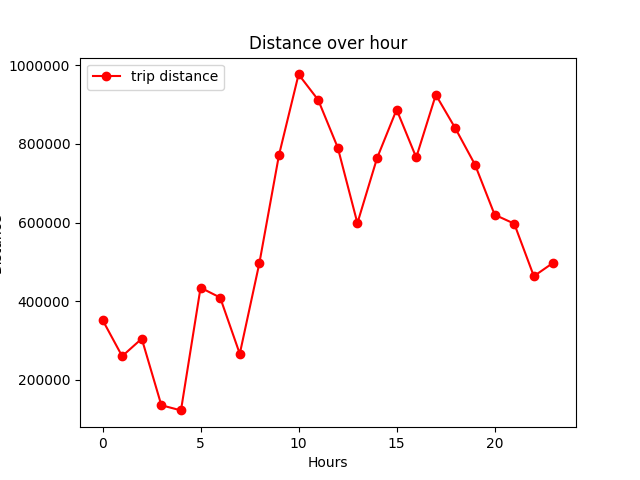
\includegraphics[width=75mm]{Figures/distance_by_day.png}
		\captionof{figure}{Evolution des distances totales par heure}
	\end{minipage}
	
	On remarque par exemple que pour le 09/09/2013 le flux des taxi est plus important entre 10h et 14h. Il faudra néanmoins faire plusieurs requêtes pour pouvoir généraliser cette règle.\\
	Notons ici que pour obtenir les données d'un mois il faudra itérer et interroger notre base 30 fois, c'est a dire interroger 30 partitions (une partition par jour).
	\subsection{Trip2}
	Nous souhaitons obtenir le nombre de trajets qui ont été pris à une "zone" donnée  (le pavé) durant une année définie. La requête utilisée est illustrée ci-dessous,
	\begin{lstlisting}
	SELECT month, daytype, pavelong, pavelat, tripid FROM TRIP2 WHERE year=2013 AND pavelong=-8.1 AND pavelat=41.1
	\end{lstlisting}
	Le résultat renvoyé par cette requête est affiché par le tableau qui suit:
	\begin{center}
		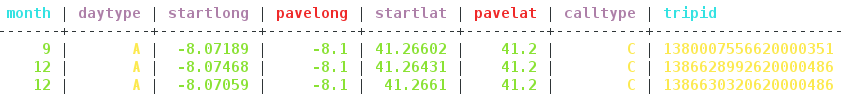
\includegraphics[width=85mm]{Figures/pave.png}
	\end{center}
	Notons qu'ici aussi nous n'utilisons ni \textit{GROUP BY} ni le \textit{COUNT}. Les trajets seront comptés dans le script Python.
	
	\subsection{Trip3}
	Pour obtenir le nombre de trajets par mois d'un taxi il faut qu'on précise son id dans la requête. On utilise pour cela une table taxi qui va stocker les ids des taxis. Ainsi il suffit juste d'itérer sur les id et concaténer l'id a la requête interrogeant la table TRIP3 comme il est illustré ci-dessous:
	\begin{lstlisting}
	query_taxi = session.execute("SELECT id FROM TAXI;")
	for user_row in query_taxi : 
	"SELECT COUNT(tripid) FROM TRIP3 WHERE year=2013 AND month=9 AND taxiid=" +str(user_row.id)+ ";"  
	\end{lstlisting}
	Nous avons essayé de représenter graphiquement les résultats sous forme d'histogramme. Ceci n'est qu'un exemple d'affichage, il sera bien évidemment amélioré avec l'avancement du projet en utilisant des librairies de Python plus adaptées.
	\begin{center}
		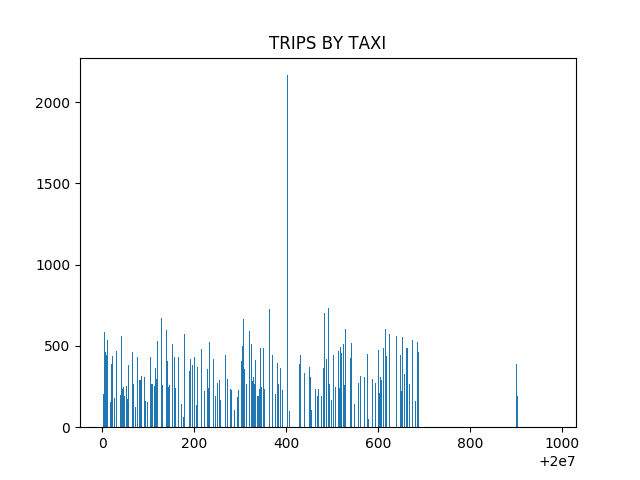
\includegraphics[width=85mm]{Figures/histogram_trip_by_taxi.png}
	\end{center}
	\subsection{Trip4}
	Nous abordons la même démarche que pour les taxi pour questionner et représenter le nombres de trajets qui ont été pris à chaque stations pour un mois donné.
	\begin{center}
		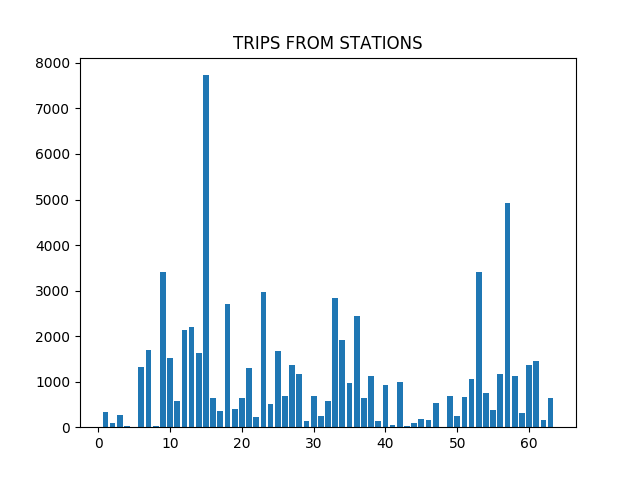
\includegraphics[width=85mm]{Figures/histogram_trip_from_station.png}
	\end{center}
	
	\subsection{kmeans}
	\subsubsection{Implémentation}
	Pour pouvoir visualiser les trajets dans une carte il faudrait pouvoir les regrouper selon des critères. Nous utilisions pour cela  les kmeans qui est une méthode non supervisée permettant de regrouper les trajets par \textit{cluster}. \\
	Nous choisissons dans notre cas de regrouper les trajets qui se ressemblent en terme de point de départ et d'arrivée. Ainsi nous avons 2 variables explicatives [startLong, startLat] et [endLong, endLat].
	La méthode des kmeans consiste a partir de centroïdes initialisés au départ par des points de notre ensemble $\Omega$ et calculer de nouveaux centroïdes qui minimisent l'inertie intra-classe. Nous supposons ici que la distance d'un point par rapport à un centroïde est calculée en sommant la distance par rapport à la variable 1 et la distance par rapport à la variable 2.\\
	Les fonctions implémentées dans la librairie de Python ne sont pas forcément faite pour traiter de gros jeux de données comme le nôtre, ainsi il est plus conseillée d'implémenter nous même la fonction des kmeans. Pour des soucis d'optimalité nous avons choisi de ne pas garder les points en mémoire car cela peut être très coûteux. Ainsi on interroge notre base de données à chaque itération pour récupérer nos points. Par conséquent, le calcul  des coordonnées de chaque centroïde se fait en sommant les coordonnées des points qui lui sont les plus proches. \\
	Les étapes de l'algorithme sont  ci-dessous:
	\begin{enumerate}
		\item Initialisation des centroïdes par des points de l'ensemble $\Omega$
		\item Tant que les nouveau centroïdes calculés sont différent des précédents, Faire:
		\begin{enumerate}
			\item une requête SELECT pour récupérer tous points
			\begin{enumerate}
				\item pour chaque point(i) calculer sa distance aux centroïdes et choisir la distance minimale
				\item sommer les coordonnées du centroïde le plus proche avec ceux du point(i)
			\end{enumerate}
			\item Calcul des nouveaux centroïdes (en divisant les coordonnées obtenus par somme par le nombre de points)
		\end{enumerate}
	\end{enumerate}
	
	Voilà ci dessous les critères pris en compte lors de l'implémentation de l'algorithme:
	\begin{itemize}
		\item Nous initialisons nos centroïdes en choisissant au hasard, grâce à  la fonction \textit{randint}, des points de notre ensemble. 
		\item Nous gardons en mémoire les centroïdes de l'itération précédente pour pouvoir tester la convergence de l'algorithme.
		\item Nous définissons le nombre de \textit{clusters}  à 3
	\end{itemize}
	
	Notre fonction kmeans retourne les centroïdes minimisant l'inertie intra-classe pour cette initialisation des centroïdes. Ainsi les kmeans trouvent un minimum local de l'inertie intra-classe. Il nous reste ensuite que d'affecter chaque observation au centroïde le plus proche pour former des clusters. Pour cela on calcule la distance de chaque point aux 3 centroïdes et on affecte celui-ci au centroïde dont il est le  plus proche.\
	
	Le code de ces 3 fonctions (\textit{distance(), kmeans() et cluster()})est à trouver en annexe dans le fichier \textit{kmeans.py}. La fonction cluster prend en paramètre la requête. Cette fonction fait appel à la fonction kmeans pour récupérer les centroïdes ensuite et affecte chaque observation à un cluster et retourne une liste avec 3 listes. Chaque sous-liste contient les points de ce cluster.\\\\
	Dans la section qui suit nous avons testé notre fonctions et avons essayé de représenter les résultats obtenus.
	
	\subsubsection{Performance, résultats et extension}
	Nous avons essayé de comprendre la différence entre les trajets pour un même jour à 10h du matin et 20h du soir. Nous représentons ci-dessous les graphes obtenus après les kmeans. La représentation est faite selon la longitude et la latitude de départ.\\
	\begin{minipage}{.5\textwidth}
		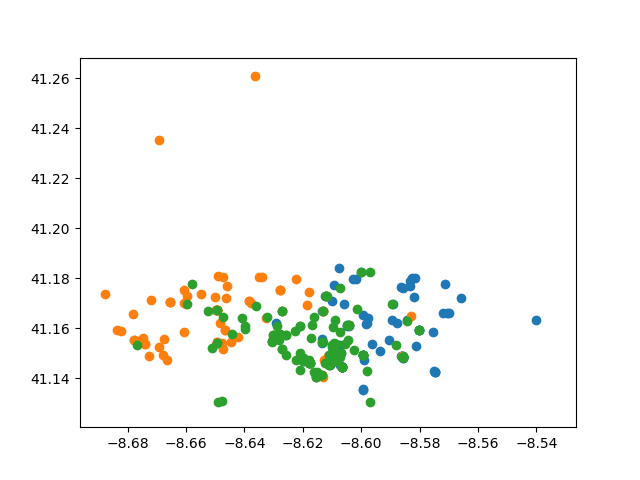
\includegraphics[width=65mm]{Figures/kmeans_10AM.png}
		\captionof{figure}{Clustering des trajets de 10h du matin}
	\end{minipage}%
	\hspace{0.02\linewidth}
	\begin{minipage}{.5\textwidth}
		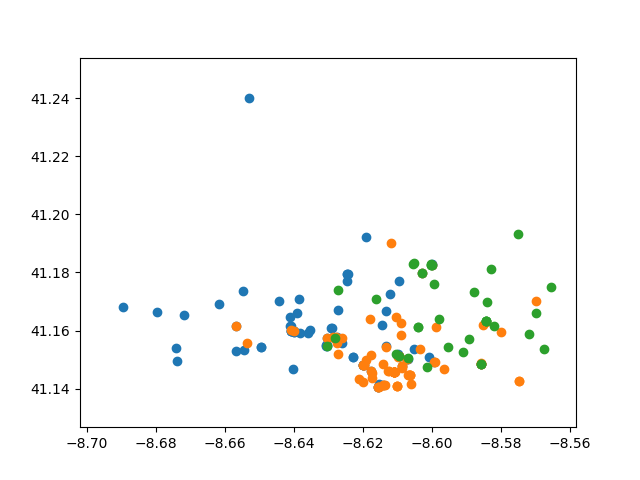
\includegraphics[width=65mm]{Figures/kmeans_8PM.png}
		\captionof{figure}{Clustering des trajets de 20h du soir}
	\end{minipage}
	
	En raison du temps cours que  nous avons eu pour développer ce projet, nous avons d'abord essayé de développer un modèle qui marche, voici donc des points que nous  serons amené à  améliorer dans la suite pour de meilleures résultats:
	\begin{itemize}
		\item \textbf{Initialisation des centroïdes:} Comme la méthode des kmeans trouve le minimum local selon l'initialisation des centroïdes, il serait judicieux de faire plusieurs appel de la fonction jusqu'à trouver l'initialisation qui minimise le critère d'inertie intra-classe.
		\item \textbf{Nombre de clusters:}  Il serait judicieux de tester avec différents nombre (entre 2 et 5 par exemple)et choisir celui qui minimise le critère d'inertie intra-classe  (exemple par methode de Cross Validation).
		\item \textbf{Paramètres:} On pourrait éventuellement changer les paramètres de la fonction \textit{cluster}() pour que celle ci prenne en paramètre que les valeurs de clés de partitionnement  et clustering (l'année, le mois le jour et l'heure)
		\item \textbf{Affichage:} Nous n'avons malheureusement pas pu installer les librairies Python (\textit{folium}) sur les postes de l'UTC qui nous auraient permis de visualiser les données sur la carte.
		\item \textbf{CQL User Defined Function (UDF):} En lisant la documentation \textit{datastax} il s'est avéré qu'on peut écrire des fonctions sur CQL en utilisant le code Python (LANGUAGE Python). On pourra alors utiliser cette méthode de classification automatique directement en interne sans avoir à récupérer les données.
	\end{itemize}
	
	\section{Conclusion}
	Ce premier mois de travail sur le projet nous a permis de faire une conception détaillée de notre base de données. Ainsi nous avons pu mettre en place différentes questions qui nous ont permis de modéliser les tables de faits correspondantes. Après nettoyage et insertion des données nous avons pu visualiser les réponses à ces questions. La méthode des kmeans nous permet de mieux étudier les flux des taxi et les visualiser.\\
	Dans la suite du projet nous serons amené à améliorer cette méthode des kmeans et développer d'autres méthodes de discrimination plus performante comme la régression logistique.
	
	\pagebreak
	
	\section{Annexe}
	Les fichiers de codes sont joints à ce rapport dans le dossier code, et sont aussi disponible sur le lien Github suivant: \url{https://github.com/Zineb-SLAM/Taxi-Service-Trajectory}
	\begin{itemize}
		\item taxi.py : Insertion des données
		\item create\_db.cqlsh: Création des tables de faits 
		\item query\_trip1: Sélection des données dans la table de fait Trip1
		\item query\_trip2: Sélection des données dans la table de fait Trip2
		\item query\_trip3: Sélection des données dans la table de fait Trip3
		\item query\_trip4: Sélection des données dans la table de fait Trip4
		\item kmeans: fonction des kmeans
	\end{itemize}
\end{document}

